% fig_87b_mg_characteristic.tex
% TR-41: 87B operating characteristic in the I_diff vs I_rst plane
%
% Two-slope characteristic:
%   Slope 1 = 30% for I_rst ≤ 1.0 pu
%   Slope 2 = 60% for I_rst > 1.0 pu
%   I_diff_min = 0.10 pu
%   Instantaneous high-set = 4.0 pu
%
% Operating points:
%   Internal fault (1 feeder): I_diff=0.20, I_rst=0.10 → TRIP
%   External fault max:        I_diff=0.032 (CT error), I_rst=1.60 → SECURE
%   Instantaneous:             I_diff=4.0 pu → instant trip

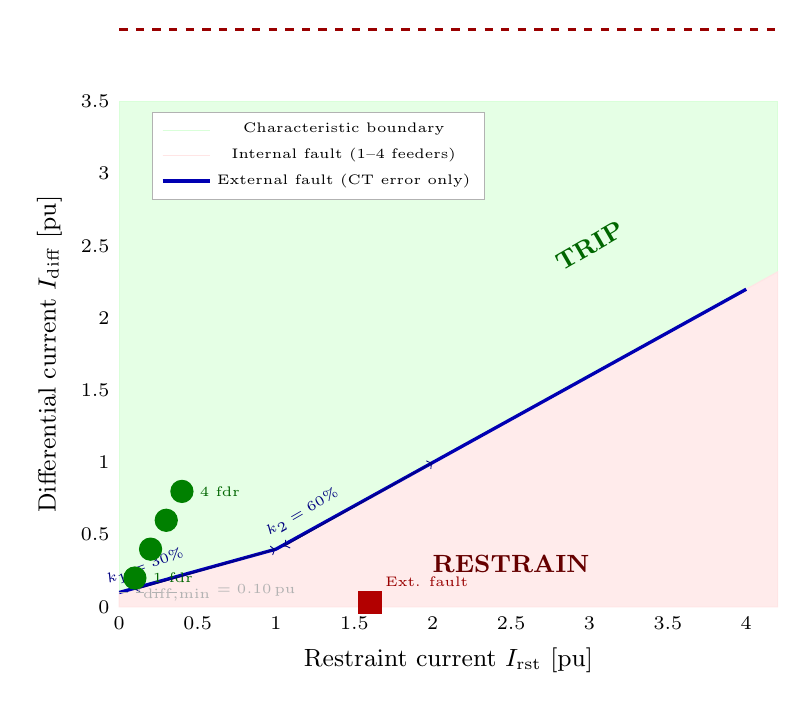
\begin{tikzpicture}
\begin{axis}[
  name         = charax,
  width        = 0.82\textwidth,
  height       = 8.0cm,
  xlabel       = {Restraint current $I_\mathrm{rst}$ [pu]},
  ylabel       = {Differential current $I_\mathrm{diff}$ [pu]},
  xlabel style = {font=\small},
  ylabel style = {font=\small},
  xmin=0, xmax=4.2,
  ymin=0, ymax=3.5,
  xtick        = {0,0.5,1.0,1.5,2.0,2.5,3.0,3.5,4.0},
  ytick        = {0,0.5,1.0,1.5,2.0,2.5,3.0,3.5},
  xticklabel style={font=\scriptsize},
  yticklabel style={font=\scriptsize},
  tick style   = {draw=none},
  axis line style={gray!50},
  grid         = major,
  grid style   = {gray!10, dashed},
  legend style = {at={(0.05,0.98)}, anchor=north west, font=\tiny,
                  draw=gray!60, fill=white},
  clip=false,
]

%% TRIP region shading (above characteristic curve)
\addplot[green!15, fill=green!10]
  coordinates {(0,0.10) (0,3.5) (4.2,3.5) (4.2,0.10)}
  \closedcycle;

%% RESTRAIN region (below characteristic)
\addplot[red!10, fill=red!8]
  coordinates {(0,0) (0,0.10) (1.0,0.40) (2.0,1.00) (3.0,1.60) (4.0,2.20) (4.2,2.32) (4.2,0) (0,0)}
  \closedcycle;

%% Operating characteristic boundary
\addplot[blue!70!black, very thick]
  coordinates {
    (0.00, 0.100)
    (1.00, 0.400)
    (2.00, 1.000)
    (3.00, 1.600)
    (4.00, 2.200)
  };
\addlegendentry{Characteristic boundary}

%% Instantaneous high-set
\addplot[red!60!black, very thick, dashed]
  coordinates {(0, 4.0) (4.2, 4.0)};
% (outside plot range — shown as text annotation)

%% Operating points — internal faults
\addplot[green!50!black, only marks, mark=*, mark size=4pt]
  coordinates {
    (0.100, 0.200)
    (0.200, 0.400)
    (0.300, 0.600)
    (0.400, 0.800)
  };
\addlegendentry{Internal fault (1--4 feeders)}
\node[green!40!black, font=\tiny, right=3pt] at (axis cs:0.100, 0.200)
  {1 fdr};
\node[green!40!black, font=\tiny, right=3pt] at (axis cs:0.400, 0.800)
  {4 fdr};

%% Operating point — external fault (CT error only)
\addplot[red!70!black, only marks, mark=square*, mark size=4pt]
  coordinates {(1.600, 0.032)};
\addlegendentry{External fault (CT error only)}
\node[red!60!black, font=\tiny, above right=2pt] at (axis cs:1.600, 0.032)
  {Ext. fault};

%% Region labels
\node[green!40!black, font=\small\bfseries, rotate=30]
  at (axis cs:3.0, 2.5) {TRIP};
\node[red!40!black, font=\small\bfseries]
  at (axis cs:2.5, 0.30) {RESTRAIN};

%% Slope annotations
\draw[<->, blue!50!black, thin]
  (axis cs:0.1, 0.12) -- (axis cs:1.0, 0.40);
\node[blue!50!black, font=\tiny, rotate=20, above left=2pt] at (axis cs:0.55, 0.26)
  {$k_1=30\%$};

\draw[<->, blue!50!black, thin]
  (axis cs:1.05, 0.42) -- (axis cs:2.0, 1.00);
\node[blue!50!black, font=\tiny, rotate=30, above left=2pt] at (axis cs:1.55, 0.71)
  {$k_2=60\%$};

%% I_diff_min
\draw[gray!60, thin, dashed]
  (axis cs:0, 0.10) -- (axis cs:0.4, 0.10);
\node[gray!60, font=\tiny, right=2pt] at (axis cs:0.0, 0.10)
  {$I_\mathrm{diff,min}=0.10$\,pu};

\end{axis}
\end{tikzpicture}
